\documentclass{article}
\usepackage[utf8]{inputenc} %codification of the document
\usepackage{float}
\usepackage{graphicx}
 \usepackage[spanish]{babel}
 
\usepackage{comment}
 
%Here begins the body of the document
\begin{document}
\section{Descripción general de la competencia}

\begin{figure}[H]
\centering
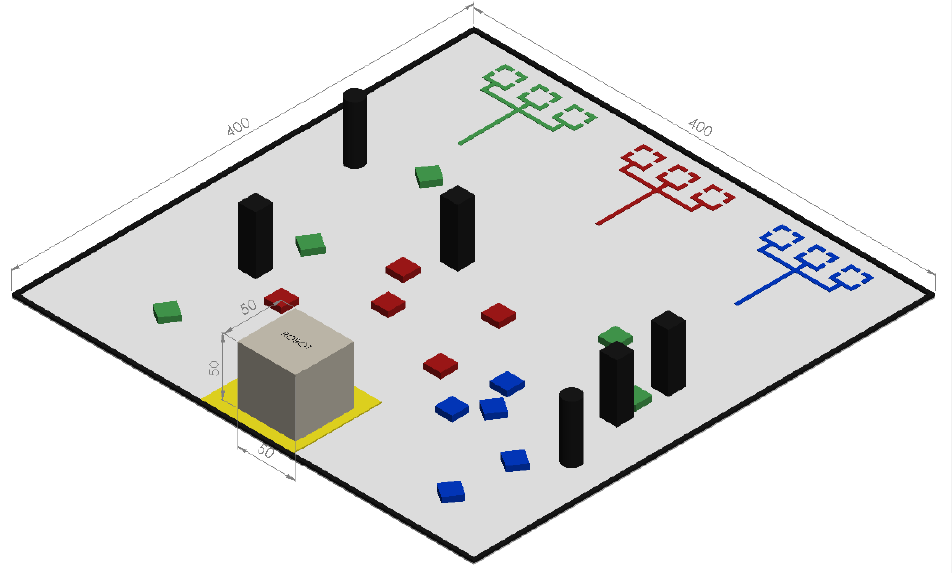
\includegraphics [scale=0.4]{descripcion}
\caption{Arena / Área de la competencia}
\end{figure}
 
\subsection{Dimensiones y peso del robot}
El tamaño (largo x ancho x alto) del robot no debe ser mayor de 50 cm x 50 cm x 50 cm. El peso no debe ser más de 20 kg, incluidas las baterías.

\subsection{Arena}
La arena es un área delimitada (4mts x 4mts), emulando una parte de un campo industrial con un terreno plano, delimitado con una línea negra de 3cm de ancho.

\subsection{Objetivo, consideraciones y reglas principales de la competencia}

\subsubsection{Objetivo:} Encontrar un objeto, clasificarlo según su color y colocarlo en la ubicación correcta de la arena; evitando a toda costa colisionar con los obstáculos. 

\subsubsection{Consideraciones: }

\begin{itemize}
    \item La figura 1 ilustra tres zonas de descarga coloreadas (rojo, azul o verde) donde el robot colocará los objetos según su color.
    \item Las líneas de las zonas de descarga tienen 3 cm de ancho y cada zona de descarga posee tres ranuras.
    \item Los objetos se distribuirán al azar dentro del escenario: 15 objetos a recoger(5 de cada color) y seis obstáculos.
    \item Tamaño de los objetos: 15cm x 15cm x 5cm.
    \item Forma y tamaño de los obstáculos: La forma del obstáculo puede ser un prisma rectángular o un cilindro. En la base miden 15cm x 15cm (prisma rectangular) o 15 cm de diámetro (cilindro). La altura de cualquier obstáculo no es menor a 15 cm.
\end{itemize}

\subsubsection{Reglas principales: }

\begin{itemize}
    \item El robot debe comenzar y terminar en el área pintada de color amarillo de 80 cm x 80 cm.
    \item Los objetos deben colocarse dentro de la ubicación correcta de manera que ambos colores correspondan.
    \item No se pueden disponer dos objetos horizontalmente sobre una misma ranura. Pero sí se pueden apilar de forma vertical.
\end{itemize}

\section{Descripción de los componentes necesarios}

Para lograr el objetivo y cumplir con las reglas de la competencia se hizo un análisis minucioso de los componentes necesarios. La siguiente lista muestra una descripción breve de su utilidad dentro del proyecto:

\subsection{Material electrónico}

\begin{itemize}
    \item Bateria LiPo: almacena una gran cantidad de energía; la suficiente para darle vida a nuestro robot.
    \item Cargador Balanceador LiPo: como durante la competencia hay rounds, entre cada round dependiendo del voltaje que tenga nuestra batería lipo recargaremos esta las veces necesarias, así como para hacer pruebas antes de la competencia.
    \item Multiadaptador p/batería LiPo: Acomodará los elementos de distinto uso o entrada.
    \item Monitor de voltaje p/batería LiPo: nos servirá para conocer el voltaje actual de nuestra batería lipo para saber en qué momento la recargaremos.
\end{itemize}

Fabricaremos un circuito impreso cuya función será controlar la velocidad y sentido de giro de los motores de nuestro robot por medio de los siguientes materiales electrónicos:

\begin{itemize}
    \item MOSFET, acopladores, resistencias, base para circuito, bloque terminal y placa fenólica de cobre.
    \item Arduino Uno R3 Genérico: este dispositivo nos ayudará a unir la programación de cada dispositivo en el robot.
    \item Protoboard: sirve para hacer pruebas antes de hacer las placas oficiales para que no tengamos que desperdiciar material si algo sale mal.
    \item Modulo Pololu: este dispositivo nos ayudará a controlar que tanto abrirá la pinza o gripper en grados así como su programación.
    \item Raspberry Pi 3 B+: hará el procesamiento de imágenes de nuestra cámara pixy.
    \item Disipador TO-22: ayudará a que los componentes no se quemen en nuestros circuitos.
    \item Cable Calibre: está aislado y su principal función es hacer conexiones.
    \item Alambre Calibre: no está aislado y su principal función es hacer conexiones.
\end{itemize}

\subsection{Sensores}

\begin{itemize}
    \item Cámara Pixy CMUcam5: cámara que ayuda a localizar los objetos por su color, conoce la distancia a la que se encuentran, así como la longitud y altura de cada objeto, está debe ser programada.
    \item Acelerómetro Analógico de 3 Ejes: determina el ángulo de inclinación y, por tanto, la posición del nuestro robot.
    \item Giroscopio Analógico: sirve para medir, mantener o cambiar la orientación en el espacio de nuestro robot.
\end{itemize}

\subsection{Actuadores}

\begin{itemize}
    \item Kit de Pinza Estándar: está pinza realizará la tarea de tomar los objetos y colocarlos dentro del robot de una manera correcta ya que también estará programada.
    \item Servo Hitec HS-422 Estándar: servirá para hacer el movimiento de la cámara para que tenga mas visión nuestro robot.
    \item Motor DC Alto Par Torque: este motor es para mover nuestras 4 ruedas omnidireccionales.
    \item Motor a pasos NEMA 17: su funcionalidad abrir y cerrar la pinza/gripper.
    \item Omnidirectional Wheel: estas ruedas son especiales ya que le permitirán a nuestro robot moverse en cualquier dirección del espacio.
\end{itemize}



\subsection{Herramientas}

\begin{itemize}
    \item Cautín: herramienta eléctrica sencilla que posee un conjunto de elementos que al estar correctamente conectados van a generar en una barra de metal el calor suficiente para poder derretir el estaño para soldar.
    \item Desoldador de Succión: es un aspirador de estaño, una herramienta de apoyo al proceso de soldadura o desoldadura.
    \item Soldadura: será de estaño y esta permite la realización de conexiones entre conductores.
    \item Pinza de Corte: servirá para cortar los cables que utilizaremos de manera correcta y más fácil.
    \item Desarmadores Kit, juego dados, pack tornillos y tuercas y pinza de punta: Herramientas que nos facilitarán la tarea de ensamblar/desensamblar el robot.
\end{itemize}


\section{Presupuesto del robot, viajes y hospedaje}

En la siguiente página se muestra una tabla con los precios de los componentes descritos anteriormente, así como el enlace correspondiente a la página del proveedor para corroborar el precio. Los precios en dólares estadounidenses (USD) se calcularon a fecha del 13 de mayo, cuando el valor era de \$19.1043.\\

Después del presupuesto del robot se muestran alternativas de vuelos y hospedajes cerca de la zona dónde se realizará el evento.


\begin{comment}
This text won't show up in the compiled pdf
this is just a multi-line comment. Useful
to, for instance, comment out slow-rendering parts
while working on a draft.
\end{comment}
 
\end{document}
